\subsubsection{Model architecture}
\label{sub:comb_model_architecture}

This sections outlines how the specific architectures for multi-input models
were determined.
Firstly, requirements and ideas for working with textual input data
are discussed.
Secondly, the experimentation process for model selection is described in detail.

The basic intuition behind incorporating tweet content into the network is to
derive more powerful content features, e.g., sentiment or recurring linguistic
patterns.
These features can then be used in conjunction  with the structured features used in previous
chapters which mainly represent contextual features about the tweet author.
This two-step process can be mapped onto a multi-input network architecture,
where sequences are processed in order to learn content features, before
merging in auxiliary contextual features, and combining both types via fully-connected
layers.
The question arises how to process textual input data most effectively.
Chapter~\ref{sub:dl_app_nlp} introduced recurrent (RNN) and convolutional neural
networks (CNN) as the most popular architectures for natural language processing tasks.
These layer architectures require input data to be temporally or locally dependent,
i.e., neighboring input features of one particular example are in some way related.
This is clearly given for sequences, as singular words only make sense
in combination with their surrounding context.
RNNs and CNNs process textual inputs in different ways.
Convolutions aim to learn features from small subsets of input data, e.g., a
fixed number of successive words (also known as \textit{filter size}).
Contrary, RNNs consume the input sequence word-by-word and learn representations
for the complete sequence.
This enables modeling of long-term dependencies in text, e.g., detection of
opening and closing brackets or subject identification.
In practice, training RNNs is more time-consuming since processing is obviously less
parallelizable.
This work focusses uses LSTM cells (see ch.~\ref{sub:dl_architectures}), because
it is the most widely adopted cell type for RNNs.
For CNNs, one-dimensional convolutional layers are applied, as textual input is
also represented as a one-dimensional list of word IDs.
Furthermore, input sequences are padded to a length of 32, and a 100-dimensional
word embedding is used.
As mentioned in Chapter~\ref{sec:data_collection}, collected data sets are
comparably small for such a complex NLP task.
As a results, model architectures have to be kept simple in order to avoid
overfitting, mainly by restricting the number of layers and cells.

\begin{figure}[h]
\begin{subfigure}{.5\textwidth}
  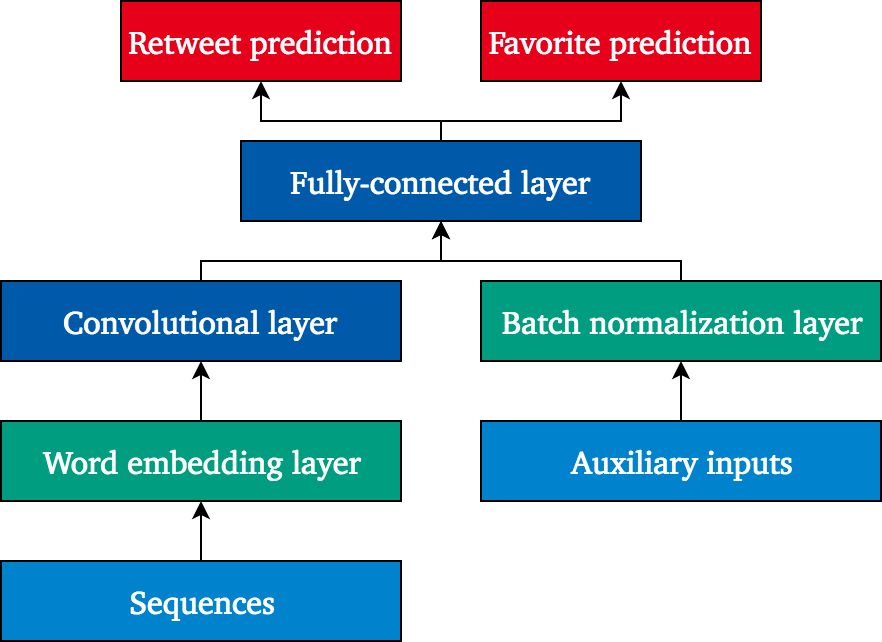
\includegraphics[width=.95\linewidth]{img/dm2_cnn}
  \caption{DM2-CNN}
  \label{fig:dm2_cnn}
\end{subfigure}%
\begin{subfigure}{.5\textwidth}
  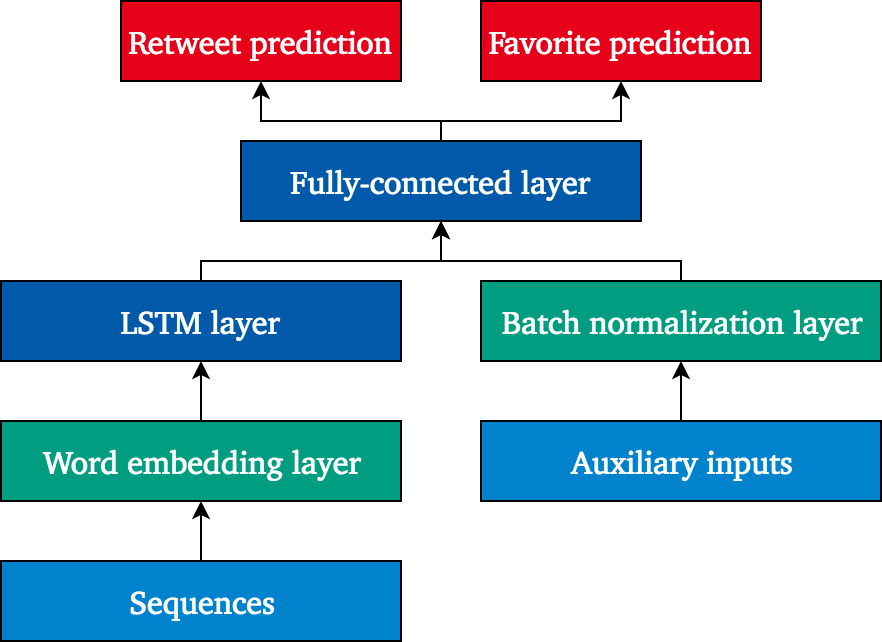
\includegraphics[width=.95\linewidth]{img/dm2_lstm}
  \caption{DM2-LSTM}
  \label{fig:dm2_lstm}
\end{subfigure}
\begin{subfigure}{.7\textwidth}
  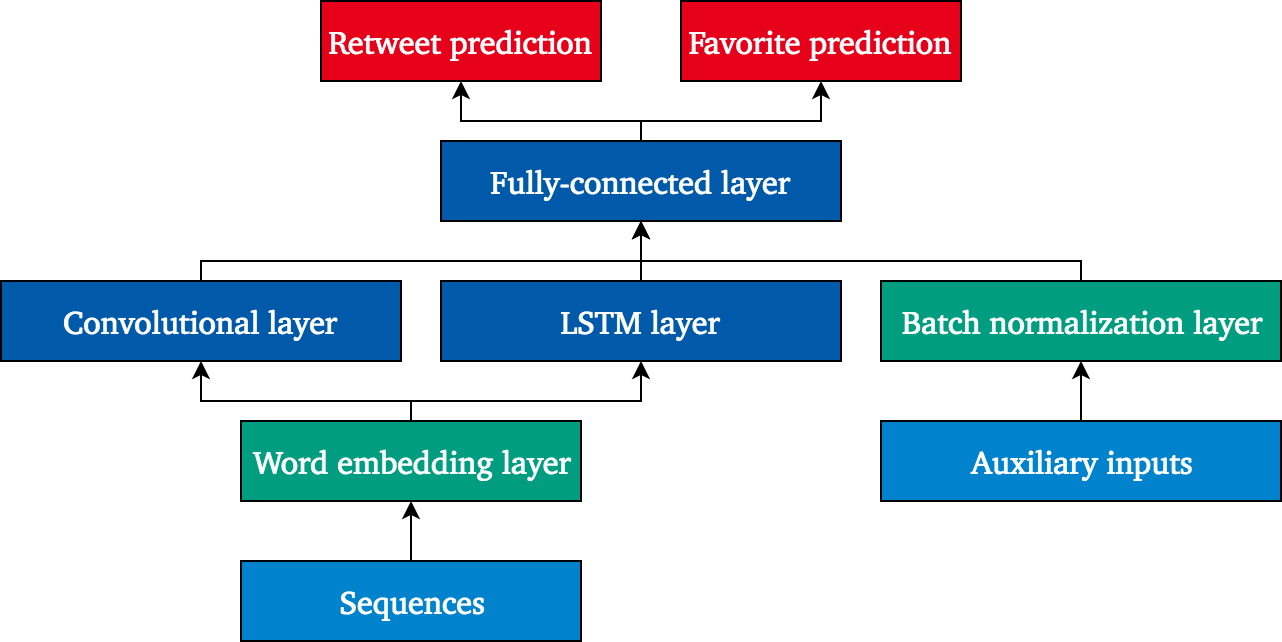
\includegraphics[width=.95\linewidth]{img/dm2_cnn_lstm}
  \caption{DM2-CNN-LSTM}
  \label{fig:dm2_cnn_lstm}
\end{subfigure}
\caption{Subset of evaluated architectures for multi-input models}
\label{fig:dm2_architectures}
\end{figure}

\structure{Model selection process}
\outline{Figure shows subset of tested architectures}
\outline{DM2-CNN applies single convolutional layer to sequences}
\outline{32 filters with size 3, padding before (keep sequence length) and max-pooling after conv layers}
\outline{DM2-CNN2 \& DM2-CNN3: same concept, but consecutive conv layers, enables
detection of more complex features, max-pooling after each layer (sequence
gets halved everytime)}
\outline{DM2-LSTM returns sequences, i.e., learned representation after each
input of the sequence (16-dimensional)}
\outline{DM2-CNN-LSTM combines both architectures, i.e., more features to combine}
\outline{Use of regularization: partly dropout after convolutions, batch
normalization after FC layer and for normalizing aux inputs}

\begin{table}
\begin{tabular}{llrr}
\toprule
Model architecture & Data set & Classification loss & Regression loss \\
\midrule
DM2-CNN & Combined & 0.7897 & \textbf{401.5174} \\
DM2-LSTM & Combined & 0.7628 & 411.2176 \\
DM2-CNN-LSTM & Combined & \textbf{0.7556} & 410.8704 \\
DM2-CNN2 & Combined & 0.7641 & 409.1842 \\
DM2-CNN3 & Combined & 0.8050 & 404.9901 \\
\bottomrule
\end{tabular}
\caption{Summary of multi-input model selection}
\label{tab:dm2_selection_results}
\end{table}

\structure{Selection results}
\outline{Selection was done on combined data set, since least prone to overfitting}
\outline{Architectures show similar performance, differences are not that big}
\outline{DM2-CNN chosen for regression: no regularization, 64 FC units}
\outline{DM2-CNN-LSTM chosen for classification: regularized via dropout after
conv layer, 128 FC neurons (intuitive since more features need to be combined)}
